\chapter{Protocollo di localizzazione}

\section{Descrizione del protocollo}
Il protocollo di localizzazione realizzato rientra nella categoria dei protocolli di localizzazione "a due vie" (Two-Ways Ranging Protocols), nello specifico alla categoria dei sistemi di posizionamento LBL (vedi par. 1.2.1).\newline Difatti il funzionamento del protocollo richiede che il nodo mobile, di cui si vuole conoscere la posizione, effettui una richiesta di localizzazione in modalita' broadcast. I nodi fissi della topologia, ricevuta la richiesta, rispondono ciascuno in modalita' "unicast" al nodo mobile (data la natura del mezzo trasmissivo, le risposte vengono ovviamente ricevute da molti nodi presenti nella topologia, ma vengono scartate discernendo rispetto al destinatario della risposta).  Una volta collezionate un minimo di 3 riposte, il nodo mobile, conoscendo a priori la posizione dei nodi fissi e potendo calcolare la propria distanza da ciascuno di essi attraverso i dati contenuti nell'header delle risposte ricevute, puo' cosi' calcolare la propria posizione tramite triangolazione, in maniera del tutto simile al funzionamento di un localizzatore GPS.

A livello dello stack dei protocolli di rete, il protocollo di localizzazione si inserisce al livello MAC, posto direttamente sopra il protocollo di livello fisico. Data la possibilita' fornita da SUNSET di far collaborare diversi protocolli per uno stesso livello dello stack protocollare, e' possibile affiancare il protocollo di localizzazione a protocolli MAC veri e propri (es. Slotted Aloha), che si occuperanno dell'effettivo accesso al mezzo. Il protocollo di localizzazione, nel caso l'AUV richieda di calcolare la propria posizione, non fa altro che aggiungere un header al pacchetto in maniera trasparente al resto della pila protocollare.

\subsection{Dettaglio degli headers protocollari}
Il protocollo utilizza due differenti headers, rispettivamente  per l'invio di richieste e risposte di localizzazione.
\newline
Per quanto riguarda l'header impiegato nella richiesta, esso si compone di 3 campi:
\newline

\begin{bytefield}[bitwidth=1.1em]{32}
        \bitheader{0-31} \\
            \bitbox{8}{SRC} & \bitbox{8}{DST} & \bitbox{16}{PKTID} \\
\end{bytefield}

\begin{itemize}
    \item sorgente della richiesta (SRC)
    \item destinazione della richiesta (DST)
    \item id della richiesta (PKTID)
\end{itemize}


I primi due campi contengono banalmente un identificativo del nodo che genera la richiesta di localizzazione e l'indirizzo dei nodi a cui la richiesta e' destinata (l'indirizzo di broadcast). Il terzo campo contiene un id univoco della richiesta (necessario per la corrispondenza fra i pacchetti di risposta e la richiesta per cui sono stati generati).\par
Per quanto riguarda l'header per il pacchetto di risposta, esso contiene i seguenti campi:
\newline



\begin{bytefield}[bitwidth=1.1em]{32}
        \bitheader{0-31} \\
        \bitbox{8}{SRC} & \bitbox{8}{DST} & \bitbox{16}{PKTID} \\
            \bitbox{16}{DEFERTIME} \\
\end{bytefield}

\begin{itemize}
    \item sorgente della risposta (SRC)
    \item destinazione della risposta (DST)
    \item id della richiesta per cui e' generata la risposta (PKTID)
    \item tempo d'attesa della risposta presso il nodo fisso (DEFERTIME)
\end{itemize}
I campi SRC e DST hanno funzione analoga a quelli presenti nell'header della richiesta ma, nel caso della risposta, il campo destinazione non conterra' l'indirizzo di broadcast ma l'identificativo del nodo cui la risposta e' dedicata ( in una sorta di modalita' "unicast" ). Il campo PKTID conterra' l'id della richiesta per cui la risposta e' stata generata. In ultimo il campo DEFERTIME verra' utilizzato per salvare l'intervallo di tempo che trascorre fra l'istante in cui il nodo fisso riceve la richiesta e l'istante in cui invia la risposta.\newline
In questo modo l'AUV, una volta effettuata una richiesta di localizzazione e ricevute delle risposte dai nodi fissi, 
sapra' calcolare, per ciascuna risposta ricevuta, la propria distanza dal nodo fisso che quella risposta ha generato.\newline Per far questo, bastera' calcolare il RTT della richiesta di localizzazione,
essendo noti l'istante di invio della richiesta, il DEFERTIME dell'header di risposta  e  l'istante di ricezione della risposta. Ovviamente, per effettuare il calcolo, dovra' essere nota anche la velocita' di propagazione di un segnale acustico in acqua, valore non costante (dipendente da una serie di fattori, fra i quali temperatura', salinita' e profondita' dell'acqua). Tuttavia e' possibile dotare un AUV  di un particolare tipo di sensori chiamati CDT (Conductivity-Temperature-Depth), che misurano appunto temperatura dell'acqua, profondita' a cui si trova il sensore e la conduttivita' del mare in quel punto (da cui e' possibile ricavare la salinita'). Conoscendo  questi fattori e' possibile ricavare una stima precisa sul valore della velocita di propagazine di un segnale acustico. 

\subsection{Esempio di funzionamento}
Viene qui descritto un esempio del funzionamento del protocollo sopra descritto.\newline Il nodo mobile, mentre e' in movimento, invia una richiesta di localizzazione, settando come indirizzo sorgente il proprio codice identificativo all'interno della topologia (tipicamente un intero univoco per ciascun nodo)
ed inserendo come indirizzo di destinazione l'indirizzo di broadcast.\newline L'AUV continuera' a muoversi mentre aspetta di ricevere le risposte dei nodi fissi. Da notare che l`AUV collezionera' solamente le risposte pervenute entro un certo intervallo di tempo dal momento di invio della richiesta (il valore di questo intervallo temporale verra' discusso nel capitolo successivo).\newline
Questi ultimi, non appena ricevuta la richiesta di localizzazione, creano il pacchetto di risposta ed avviano ciascun un proprio timer. Questo timer, il cui runtime viene calcolato a partire da una distribuzione randomica uniforme (da 0 ad un valore massimo parametrizzato), adempie al compito di desincronizzare le risposte dei nodi fissi,
facendo in modo che se si verifichino un minor numero di collisioni fra i pacchetti (essendo il mezzo condiviso).\newline Da notare, come gia' detto, che la risposta viene inviata in modalita' "unicast", settando l'indirizzo di destinazione con quello del nodo mobile che ha generato la specifica richiesta. Potenzialmente, questo meccanismo permette l'eventuale possibilita' di localizzare due o piu' nodi mobili, potendo questi ultimi discernere quali pacchetti di risposta sono a loro indirizzati.\newline
Ad ogni modo, l'AUV colleziona un certo numero di risposte a lui indirizzate e, una volta scaduto il timer d'attesa delle risposte, effettua i calcoli necessari alla propria localizzazione, a partire dal calcolo della propria distanza da ciascun nodo fisso da cui ha ricevuto riposta.\newline
Questo calcolo, nel caso del veicolo in movimento, viene condizionato da due tipologie d'errore che andranno ad inficiare il risultato finale della misurazione. 
In primo luogo, come gia' anticipato, l'AUV calcola la distanza dai nodi fissi a partire dal RTT. Questo valore viene moltiplicato per la velocita' del suono in acqua ( nel simulatore 1500 m/s) e il valore ottenuto viene quindi dimezzato.
Quest'ultima divisione presuppone che il tempo di propagazione della richiesta di localizzazione si pari a quello di propagazione della risposta, cosa non vera nel caso dell'AUV in movimento (si pensi al caso in cui il veicolo si stia dirigendo proprio verso un nodo fisso da cui riceve risposta).\newline
In aggiunta, la distanza viene calcolata al momento dello scadere del timer avviato dall'AUV non appena effettuata la richiesta di localizzazione e non quando il veicolo riceve la risposta.
Il valore della distanza ottenuto col calcolo sara' riferito a questo secondo istante temporale, mentre il calcolo della posizione del nodo mobile avviene al primo.

\subsection{Parametri d'interesse e modalita' di funzionamento del protocollo}
\subsubsection{Valore massimo del timer di desincronizzazione dei nodi fissi}
Alcuni parametri fondamentali condizionano in maniera netta il funzionamento del protocollo di localizzazione.\par Uno su tutti e' l'ampiezza dell'intervallo
in cui i nodi fissi scelgono, con distribuzione uniforme di probabilita', il tempo con cui avviare il timer necessario alla desincronizzazione dei pacchetti di risposta.
Il timer serve a far si che, con ragionevole certezza, i nodi fissi rispondano ad una richiesta di localizzazione in istanti differenti l'uno dall'altro (anche nel caso ricevano la richiesta quasi nello stesso momento).
Il valore con cui viene inizializzato il timer, come detto, viene scelto a caso in un intervallo di valori che parte da 0 ad un certo valore massimo.
Ovviamente, piu' elevato sara' il valore dell'estremo superiore di questo intervallo, maggiore sara' la scelta di valori possibili per il timer, minore la possibilita' che i nodi fissi inviino riposte in istanti fra loro vicini e quindi
piu' basso il verificarsi di collisioni fra le stesse risposte. Il maggior numero di risposte ricevute fara' si che ci sia una piu' alta percentuale di localizzazioni andate a buon fine (ricordiamo la necessita' di ricevere almento 3 risposte per effettuare il posizionamento dell'AUV).\newline
Tutto cio' a scapito della precisione nel calcolo della posizione del nodo mobile. Difatti, come anticipato nel paragrafo precedente, il veicolo mobile effettua il calcolo della propria posizione allo scadere di un timer, il cui runtime e' dato dalla somma dei seguenti elementi:
\begin{itemize}
    \item Tempi di  trasmissione e propagazione di una richiesta
    \item Tempi di  trasmissione e propagazione di una risposta
    \item L'estremo superiore dell'intervallo numerico dal quale i nodi fissi reperiscono il valore con cui avviare il timer di desincronizzazione
\end{itemize}
Piu' il calcolo avviene temporalmente tardi rispetto alla generazione della richiesta, piu' aumenta l'errore sul calcolo della posizione (per i due fattori spiegati nel paragrafo precedente).
Riportiamo di seguito due grafici esemplificativi di quanto appena spiegato ( i grafici si riferiscono ad una topologia con 6 nodi fissi, AUV in movimento ad 1$\frac{m}{s}$ e numero minimo di risposte necessarie pari a 3).
\begin{figure}[H]
    \centering
    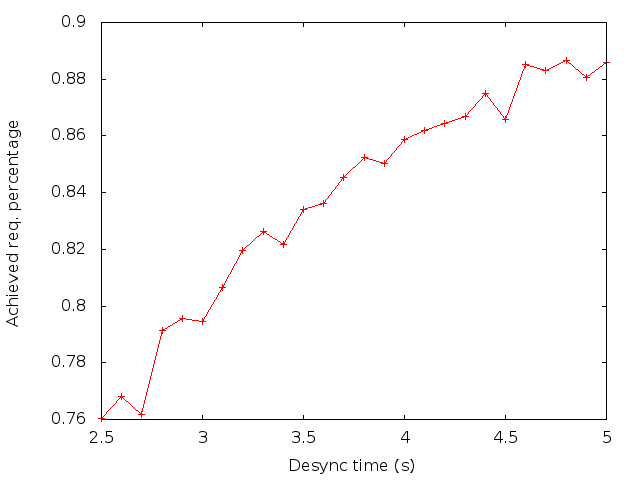
\includegraphics[scale=0.5]{achievedlochexagon6nodescutoff4req3preempt0droponepoint0speed1.png}
    \caption{Percentuale richieste andate a buon fine}
    \label{fig:my_label}
\end{figure}
\begin{figure}[H]
    \centering
    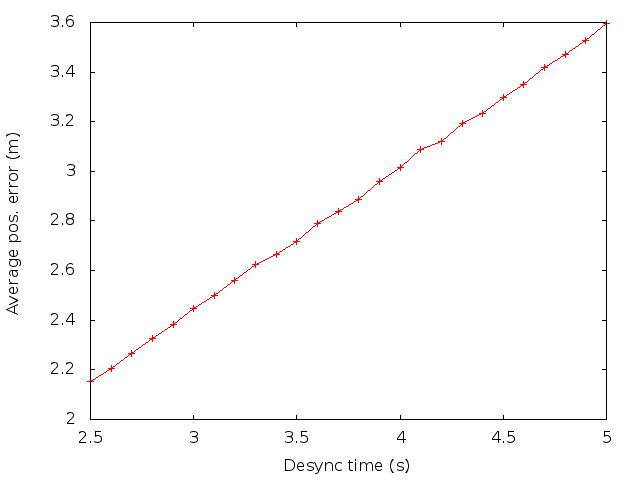
\includegraphics[scale=0.5]{avposerrorhexagon6nodescutoff4req3preempt0droponepoint0speed1.png}
    \caption{Errore medio}
    \label{fig:avposerrorhexagon6nodescutoff4req3preempt0droponepoint0speed1}
\end{figure}
I grafici mappano rispettivamente la percentuale di localizzazioni andate a buon fine e l'errore medio rispetto alla posizione reale, utilizzando come valore sull'asse delle ascisse proprio il massimo tempo di desincronizzazione possibile per i nodi fissi.\newline
\subsubsection{Numero minimo di risposte richieste}
Il funzionamento dell'algoritmo di localizzazione, come verra' esposto in seguito, fa si che' ad un maggior numero di risposte pervenute dai nodi fissi corrisponda un calcolo della posizione del nodo mobile piu' preciso.
Per valutare l'influenza del numero di risposte ricevute sulla precisione della localizzazione e' stato introdotto, come parametro di funzionamento del protocollo, il numero minimo di risposte che vengono richieste per effettuare il calcolo della posizione del nodo mobile.\newline Questo valore non puo' scendere sotto la soglia di 3, numero minimo di risposte necessarie ad effettuare il calcolo. 
Aumentare il valore di questo parametro non aumenta tanto l'accuratezza della posizione calcolata dell'AUV, ma piuttosto aumenta la consistenza del calcolo, facendone diminuire l'errore massimo generato . Tutto questo a scapito  del numero di localizzazioni andate a buon fine (ad esempio , impostando come soglia minima il valore 5, tutti i casi in cui il nodo mobile ricevera' 3 o 4  risposte verranno scartati).\newline
\begin{figure}[H]
    \centering
    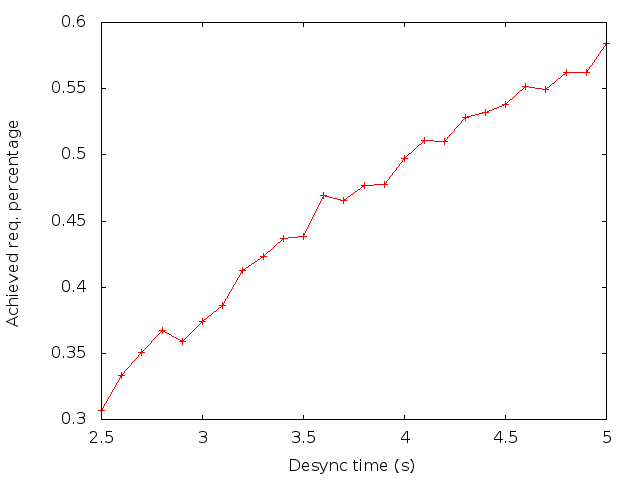
\includegraphics[scale=0.5]{achievedlochexagon6nodescutoff4req5preempt0droponepoint0speed1.png}
    \caption{La percentuale di richieste andate a buon fine diminuisce aumentanto il numero minimo di risposte richiesto (grafico per soglia minima di risposte pari a 5)}
\end{figure}

\begin{figure}[H]
    \centering
    \subfloat[3 risposte]{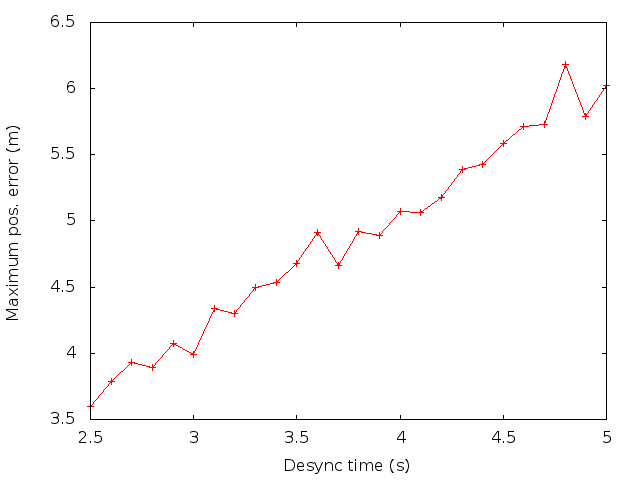
\includegraphics[width=0.4\textwidth]{maxposerrorhexagon6nodescutoff4req3preempt0droponepoint0speed1}\label{fig:f1}}
    \hfill
    \subfloat[5 risposte]{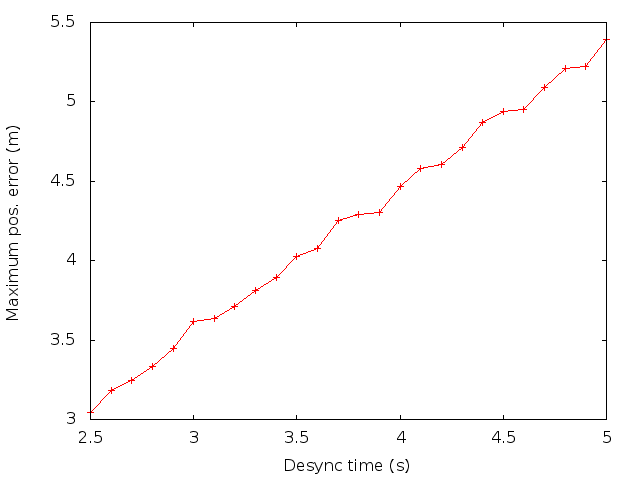
\includegraphics[width=0.4\textwidth]{maxposerrorhexagon6nodescutoff4req5preempt0droponepoint0speed1}\label{fig:f2}}
    \caption{A sinistra, l'andamento dell'errore massimo con numero di richieste minimo impostato a 3. A desta, lo stesso grafico ma con soglia minima impostata a 5. Aspettando due risposte in piu' si guadagnano 0.5 metri sull'errore massimo}
\end{figure}
\subsubsection{Soglia massima numero di condizionamento della matrice del sistema}
\par
Nel calcolo della posizione dell'AUV, ci si trova a dover risolvere un sistema lineare nella forma  \(\textbf{A}\overrightarrow{x} = \overrightarrow{b} \) , ricorrendo a metodologie di approssimazione della soluzione corretta (vedi paragrafo 3.2.4). Per la matrice \(\textbf{A}\) e' possibile definire un valore, detto numero di condizionamento, che ci fornisce una sorta di limite superiore  per l'errore che possiamo ottenere nel calcolo delle coordinate del veicolo mobile. Piu' e' elevato il valore del numero di condizionamento, maggiore e' l'errore che puo' inficiare la validita' della localizzazione. Viene quindi introdotta una soglia massima per il valore del numero di condizionamento, al di sopra della quale la specifica richiesta di localizzazione viene scartata (in modo cosi' da evitare misure influenzate da un errore elevato).
\subsubsection{Modalita' di funzionamento "preemptive"}
Contestualmente all'introduzione del parametro riguardante il numero minimo di risposte richieste, si e' pensato di realizzare una seconda modalita' di funzionamento del protocollo, che verra' indicata col nome di modalita'  ``preemptive''.\newline In questa modalita' viene modificato il  comportamento del nodo mobile rispetto all'attendere lo scadere del timer prima di iniziare il calcolo della propria posizione. Come gia' discusso, cio' comporta un aumento dell'errore nella misurazione della distanza rispetto ai nodi fissi di cui si e' ricevuta risposta, dovuta alla non contemporaneita' del calcolo della posizione rispetto alla ricezione stessa della riposta (in particolare, l'errore sara' tanto maggiore quanto prima si e' ricevuta la risposta rispetto alla fine del timer).\newline
Nella modalita' ``preemptive'' il veicolo, invece di aspettare la fine del timer,  avvia l'algoritmo di localizzazione non appena riceve il numero di risposte indicato dal parametro della soglia minima di risposte necessaria.
Riportiamo il grafico ottenuto sempre con la configurazione a 6 nodi fissi, soglia minima di risposte pari a 3 e velocita' dell'AUV fissata a 1$\frac{m}{s}$. Notiamo come, rispetto al grafico in figura ~\ref{fig:avposerrorhexagon6nodescutoff4req3preempt0droponepoint0speed1}, l'errore medio sia piu' che dimezzato rispetto alla modalita' non "preemptive"
\begin{figure}[H]
    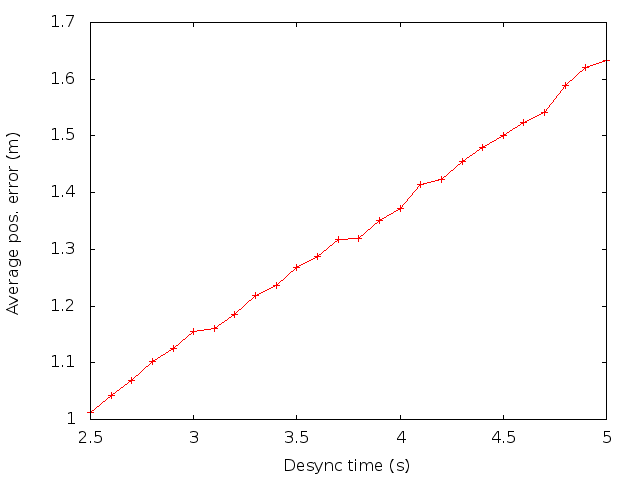
\includegraphics[scale=0.5]{avposerrorhexagon6nodescutoff4req3preempt1droponepoint0speed1.png}
    \centering
\end{figure}

\subsubsection{Modalita' di funzionamento "drop one point"}
\par
Questa modalita' di funzionamento e' strettamente legata alla soglia massima tollerabile introdotta per il valore del numero di condizionamento. Nel corso delle simulazioni, si sono riscontrati valori elevati del numero di condizionamento nei casi in cui il veicolo mobile avesse ricevuto risposte alla propria richiesta di localizzazione da un insieme di nodi nei quale tre dei sensori fissi risultassero quasi allineati sulla stessa retta. Si e' pensato quindi di introdurre una modalita' di funzionamento del protocollo in cui, invece di applicare una strict policy nel caso del superamento della soglia del condition number, l'AUV prova ad eliminare dall'insieme delle risposte ricevute quella proveniente da uno dei nodi allineati, in modo da ottenere nella localizzazione una matrice con numero di condizionamento al di sotto della soglia di guardia. Per ottenere questo risultato in maniera computazionalmente efficiente, l'AUV scarta iterativamente una delle riposte ottenute (ovviamente solo se ha ricevuto 4 o piu' risposte) e prova ad effettuare la localizzazione col sottoinsieme di risposte cosi ottenuto.
\par
In ultimo, un parametro importante nell'agire del protocollo e' la soglia minina per il valore del condition number della matrice rappresentante il sistema lineare la cui risoluzione genera la posizione calcolata dell'AUV. Questo parametro verra' discusso in dettaglio nella sezione dedicata al calcolo della posizione.\newline


\section{Calcolo della posizione}

\subsection{Descrizione generica del calcolo}
La tecnica impiegata per il calcolo della posizione fa uso della metodologia della trilaterazione. La trilaterazion e' un processo geometrico che permette il calcolo della posizione assoluta o relativa di un punto in base alla misurazione di di alcune distance (in questo caso le distanze dai nodi fissi), utilizzando la geometria delle sfere.\newline
Da specificare che, nel caso del nostro nodo mobile, considereremo come nota la profondita' dell'AUV, potendo far uso di un sensore di profondita' di notevole precisione (basato sulla pressione marina).\newline
Quindi, il nostro calcolo verra' effettuato non in tre ma in due dimensioni. 

\subsection{Impostazione matematica del calcolo}
Per ogni risposta i che l'AUV riceve da un nodo fisso, possiamo scrivere l'equazione della sfera avente come centro il nodo fisso e come raggio la distanza del veicolo mobile da quel nodo, calcolata tramite il RTT: \newline
\begin{equation}
r_{i} = \sqrt{(x-x_{i})^2+(y-y_{i})^2+(z-z_{i})^2} \qquad (i = 1,...,n)
\end{equation}
\newline
Il metodo banale di risoluzione consisterebbe nel risolvere il sistema di equazioni quadratiche, cosa computazionalmente onerosa.\newline Inoltre, a causa degli errori introdotti nella misura dei raggi delle sfere, non e' detto che il sistema dato abbia soluzione.\newline
Per rendere piu' abbordabile il calcolo, utilizzeremo delle piu' sofisticate tecniche di risoluzione, basate sulla linearizzazione del sistema e su tecniche di risoluzione approssimate.\newline

\subsection{Linearizzazione del sistema}
In primis, come gia' detto, consideriamo nota la profondita' dell'AUV, $z_{0}$, da cui:
\begin{equation}
(x-x_{i})^2+(y-y_{i})^2 = r'^2_{i} , con r'^2_{i} = r^2_{i}-(z_{0}-z_{i})^2 \qquad  (i = 1,...,n)
\end{equation}
\newline
Quindi il sistema passa da tre incognite a due sole incognite, il che fa si che avremo bisogno di un'equazione in meno per risolvere il sistema stesso.\newline
Utilizziamo indifferentemente una delle equazioni per linearizzare il sistema, in questo caso la prima equazione, da cui avremo:\newline
\begin{equation}
(x-x_{1}+x_{1}-x_{i})^2+(y-y_{1}+y_{1}-y_{i})^2 =  r'^2_{i} \qquad  (i = 2,...,n)
\end{equation}
\newline
Da cio' otterremo il seguente sistema:\newline
\begin{equation}
2(x_{1}-x_{i})+2(y_{1}-y_{i}) =  r'^2_{i}-r'^2_{1}-x^2_{i}-y^2_{i}+x^2_{1}+y^2_{1} \qquad (i = 2,...,n)
\end{equation}

A partire da un sistema di n equazioni di secondo grado in tre incognite, abbiamo ottenuto un sistema lineare in due incognite con n-1 equazioni.\newline Ora diviene chiaro il perche' della soglia minima di risposte necessarie fissata a 3, che permette in finale di ottenere un sistema lineare di due equazioni in due incognite.\newline Il sistema, nella forma $\textbf{A}\overrightarrow{x}=\overrightarrow{b}$, potrebbe essere risolto direttamente risolvendo due delle equazioni in esso presenti.\newline Cio' non e' detto sia possibile ne' ci viene garantito che si ottenga in tal modo il risultato piu' preciso.\newline Adotteremo quindi una diversa approssimata di risoluzione, nota come metodo dei minimi quadrati.\newline

\subsection{Metodo dei minimi quadrati}
Il metodo dei minimi quadrati e' un metodo di ottimizzazione il cui scopo e' individuare, dato un insieme di dati (punti del pinao), una funzione che ben si avvicini a quei dati.\newline In particolare, questa funzione sara' quella che minimizza la somma dei quadrati della differenza fra i dati osservati e i punti della funzione approssimante (da cui il nome del metodo).\newline
In questo caso, il valore da minimizzare e': \newline
\begin{equation}
S = \overrightarrow{r}^T\overrightarrow{r} = (\overrightarrow{b}-\textbf{A}\overrightarrow{x})^T(\overrightarrow{b}-\textbf{A}\overrightarrow{x})
\end{equation}
\newline
Da questa formula si arriva all'equazione normale:\newline
\begin{equation}
\textbf{A}^T\textbf{A}\overrightarrow{x} = \textbf{A}^T\overrightarrow{b}
\end{equation}
\newline
A questo punto, se la matrice non e' singolare, si puo' risolvere direttamente l'equazione:\newline
$\overrightarrow{x} = (\textbf{A}^T\textbf{A})^{-1}\textbf{A}^T\overrightarrow{b}$
La risoluzione diretta dell'equazione normale non e' detto generi risultati precisi.\newline La causa di quest'imprecisione e' da ritrovarsi nel numero di condizionamento della matrice.\newline
Il sistema lineare $\textbf{A}\overrightarrow{x} = \overrightarrow{b}$ puo' essere in realta' riscritto, per via degli errori sulla misurazione delle distanze, come: \newline
\begin{equation}
\textbf{A}\overrightarrow{x} = \overrightarrow{b} \rightarrow \textbf{A}(\overrightarrow{x}+\delta\overrightarrow{x}) = (\overrightarrow{b}+\delta\overrightarrow{b})
\end{equation}
\newline
in cui $\delta\overrightarrow{b}$ e' proprio l'errore introdotto dall'imprecisione nelle misurazioni.
In tal modo possiamo scrivere l'errore nel calcolo in forma matriciale:\newline
\begin{equation}
\textbf{A}\delta\overrightarrow{x} = \delta\overrightarrow{b}
\end{equation}
\newline
da cui: \newline
\begin{equation}
||\delta\overrightarrow{x}|| \leq ||\textbf{A}^{-1}|| \cdot ||\delta\overrightarrow{b}||
\end{equation}
Definiamo a questo punto il numero di condizionamento come la quantita': \newline
\begin{equation}
\kappa (\textbf{A}) = ||\textbf{A}|| ||\textbf{A}^{-1}|| 
\end{equation}
\newline
Finalmente giungiamo all'equazione: \newline
\begin{equation}
\frac{||\delta\overrightarrow{x}||}{||\overrightarrow{x}||} \leq  \kappa (\textbf{A}) \frac{||\delta\overrightarrow{b}||}{||\overrightarrow{b}||}
\end{equation}
Questa e' la stima dell'errore relativo che, come vediamo, dipende fortemente dagli errori presenti nelle misurazioni delle distanze che viene amplificato secondo un fattore che dipende dalla natura stessa della matrice.\newline Indipendentemente dall'errore presente nel calcolo delle distanze dai nodi fissi, un basso numero di condizionamento ci garantisce che l'errore nelle misurazioni non si propaghera' in maniera esagerata mentre, al contrario, un alto valore del condition number potrebbe rendere inutilizzabile la posizione calcolata anche in presenza di un piccolo errore sui termini noti.\newline
Viene appunto introdotto, quindi, un parametro di funzionamento del protocollo che rappresenta la soglia massima accettabile per il valore del condition number della matrice \textbf{A}, scartando i risultati in caso di superamento di tale soglia.

\section{Considerazioni sull'utilizzo e testing del protocollo}
\par
Nella sezione successiva dell'elaborato verranno presentati i dati relativi ai test di simulazione del protocollo, di cui ivi si vuole dare una breve panoramica, sottolineando in particolare quali sono stati gli obbiettivi che hanno guidato tutta la fase di testing.
\par
I parametri d'interesse nella valutazione  dell'algoritmo sono stati essezialmente tre:
\begin{itemize}
\item La percentuale di localizzazioni andate a buon fine rispetto al numero di localizzazioni tentate
\item L'errore medio ottenuto nel calcolo della posizione dell'AUV
\item L'errore massimo riscontrato nel valore della posizione calcolato
\end{itemize}
Ovviamente, obbiettivo principale delle simulazione e' stato valutare in quali configurazioni di funzionamento del protocollo si riuscisse a massimizzare la percentuale di richieste di localizzazione effettuate con successo posto che, ancor prima di considerazioni sull'errore di posizionamento, fosse importante ottenere una buona percentuale d'affidabilita' del protocollo stesso.  In secondo luogo, l'ovvia rilevanza dell'errore medio ottenuto sulla localizzazione come misura della bonta' del protocollo e di un suo eventuale utilizzo in un contesto applicativo reale. La terza misura e' stata un indicatore della varianza dell'errore insito nella localizzazione posto che, in uno scenario di concreto utilizzo del protocollo, la misurazione della posizione di un veicolo mobile puo' effere ulteriormente raffinata facendo ricorso a filtri matematici (es. filtro di Kalman) e tecniche di dead-reckoning (stima della posizione  di un veicolo in base ad una posizione precedente nel tempo e ad informazioni sul movimento del veicolo stesso).

